\documentclass[aspectratio=169]{beamer}
\usepackage{tikz}
\usetheme{Warsaw}
\title{Boxes and Columns}
\begin{document}

\begin{frame}
  \titlepage
\end{frame}

\begin{frame}{Layout stress}
  \begin{columns}[c]
    \begin{column}{0.32\textwidth}
      \begin{block}{A}
        Short A
      \end{block}
    \end{column}
    \begin{column}{0.32\textwidth}
      \begin{alertblock}{B}
        Short B
      \end{alertblock}
    \end{column}
    \begin{column}{0.32\textwidth}
      \begin{exampleblock}{C}
        Short C
      \end{exampleblock}
    \end{column}
  \end{columns}

  \vspace{1em}
  A full-width rule and a table:
  \begin{center}
    \begin{tabular}{|c|c|c|}
      \hline
      Device & $h_{FE}$ & $V_{CEO}$ \\
      \hline
      BC546 & 110--800 & 65\,V \\
      BC547 & 110--800 & 45\,V \\
      \hline
    \end{tabular}
  \end{center}
\end{frame}

\begin{frame}{Vector-ish content}
  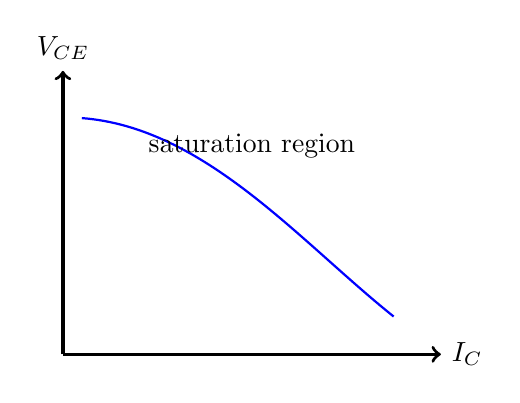
\begin{tikzpicture}[scale=1.2]
    \draw[very thick,->] (0,0) -- (4,0) node[right] {$I_C$};
    \draw[very thick,->] (0,0) -- (0,3) node[above] {$V_{CE}$};
    \draw[thick,blue] (0.2,2.5) .. controls (1.5,2.4) and (2.5,1.2) .. (3.5,0.4);
    \node at (2,2.2) {saturation region};
  \end{tikzpicture}
\end{frame}

\end{document}
